\documentclass[a4j,12pt,onecolumn,oneside,final]{jreport}

\usepackage[dvipdfmx]{graphicx}	%figure
\usepackage{subfig}
\usepackage{latexsym}
\usepackage[pdftex]{epstopdf}
%\usepackage{gthesis}
\usepackage{gthesis_myown}

\usepackage{amsmath,amsthm,amssymb,ascmac}
\usepackage{amsfonts}
\usepackage{fancybox}
\usepackage{slashbox}
%\usepackage[dviout]{color,graphics}
\usepackage{color}
\usepackage{psfrag}
%\usepackage{upgreek}
\usepackage{bm}
\usepackage{wrapfig}
\usepackage{listings}	% source code
\usepackage{balance}
\usepackage{txfonts}
\usepackage[T1]{fontenc}
\usepackage{lmodern}
\usepackage[deluxe]{otf}
\usepackage{array}
\newcolumntype{$}{>{\global\let\currentrowstyle\relax}}
\newcolumntype{^}{>{\currentrowstyle}}
\newcommand{\rowstyle}[1]{\gdef\currentrowstyle{#1}%
  #1\ignorespaces
}

\lstset{%
  language={XML},
  basicstyle={\small},%
  identifierstyle={\small},%
  commentstyle={\small\itshape},%
  keywordstyle={\small\bfseries},%
  ndkeywordstyle={\small},%
  stringstyle={\small\ttfamily},
  frame={tb},
  tabsize=4,
  breaklines=true,
  columns=[l]{fullflexible},%
  numbers=left,%
  xrightmargin=0zw,%
  xleftmargin=3zw,%
  numberstyle={\scriptsize},%
  stepnumber=1,
  numbersep=1zw,%
  lineskip=-0.5ex%
}

%%%%%%%%%%%%%%%%%%%%%%%%%%%%%%%%%%%%%%%%%%%%%%%%%%%%%%%%%%%%%%%%
% put local tex-macros in this file %

%%%%%%%%%%%%%%%%%%%%%%%%%%%%%
%色設定
%%%%%%%%%%%%%%%%%%%%%%%%%%%%%
\definecolor{Black}{rgb}{0.0,0.0,0.0}
\definecolor{Red}{rgb}{0.9,0.0,0.1}
\definecolor{Blue}{rgb}{0.1,0.1,0.5}
\definecolor{Green}{rgb}{0.1,0.4,0.1}
\definecolor{Gray}{rgb}{0.75,0.85,0.9} % Fuji-iro
\definecolor{Shade}{rgb}{0.1,0.1,0.4}

%%%%%%%%%%%%%%%%%%%%%%%%%%%%%%%%%%%%%%%%%%%%%%%%%%%%%%%%%%%%%%%%
\年度{平成26年度}
%\提出年月{平成26年7月}
\提出年月{平成27年2月}

\題名{SIBM - RDF形式に記述した避難場所情報\\ベンチマークツール}
\梗概題名{SIBM - RDF形式に記述した避難場所情報\\ベンチマークツール}
%\題名{楽に卒業する方法に関する基礎的研究\\
%			--- そもそもそれは可能か? ---}
%\梗概題名{楽に卒業する方法に関する基礎的研究\\
%			--- そもそもそれは可能か? ---}

\指導教員名A{横田 治夫}
\職名A{教授}

\指導教員名B{荒堀 喜貴}
\職名B{助教}

%\所属学科{電気電子工学科}{}
\所属学科{情報工学科}{}
\学籍番号{11\_27820}
\氏名{NGUYEN Hoai Nam}

\内容梗概{
世界中で毎年、災害による損失や市民生活への影響が問題となっている.災害発生時には、避難情報を元に避難することが必要であるが、
災害発生後に、避難に関する情報やデータの量は急速に増加する.このため、適切な災害・避難情報の管理が求められる.

一方、近年RDF形式で記述されたデータが幅広く使用され、災害情報などを含む様々なデータがRDF形式で保存されることが増えている.
RDF形式を利用すると、情報の細かな管理やアクセス制限を適切に行うことができるが、既存の災害情報のRDF表現では、被災者個人間の関係や
被災者と医者、ボランティアなどの支援者との関係や、どの支援者がどの被災者にどのような作業を行って良いかといった関係を表現できていない.

そこで、本研究では、これらの詳細な関係をRDF形式で記述した災害・避難情報のデータセットSIBMを提案する.
SIBMの目的は、被災地における被災者-支援者間のデータ共有方式の妥当性の評価を可能にすることである.
具体的には、被災者の怪我の程度などの個人情報は医療従事者にのみ開示し、他の被災者には個人情報へのアクセスを許可しないなどの
データ共有方式の性能や秘匿情報保護能力をSIBMによって計測できるようになることを目指す.}

\begin{document}
% ----------------------------------------------------------------------
% 表紙
\maketitle
% ----------------------------------------------------------------------
% 目次
\setcounter{page}{1}
\renewcommand{\thepage}{\roman{page}}
\setcounter{tocdepth}{1}
\tableofcontents
\clearpage
% ----------------------------------------------------------------------
% 内容
\setcounter{page}{1}
\renewcommand{\thepage}{\arabic{page}}
%\chapter{Introduction}
\chapter{序論}
全世界には 、毎年災害が沢山発生する.大規模災害の2011年の大震災の他 、台風による災害事故や土砂災害などによる破壊が多いとわかった.
災害が発生するとき、避難することは重要である.避難する際、避難場所情報の管理や、避難する作業に関係のある人々の情報が多量に増加することがある.
それらの情報を管理・アクセスすることが重要な作業である.現実では、避難することに関する情報の中に、避難場所情報、
避難する人の情報、避難場所で作業する人(アシスタント・ボランチアなど)の情報があり、それらの情報を管理・アクセスすることが考えられる.
災害が発生するとき、それらの情報に対してすぐに対応できることが重要である. そのため、災害対策作業に対して、
現実に近い情報を使用しながら実験することは実際の要求である.

	一方、近年には、様々な新たなデータ記述法が開発されている.その中に、RDF形式で記述されたデータが増えている.
RDF形式で記述された避難・災害情報を公開・管理することが考えられている\cite{cite:opendata}.
RDF形式で記述したデータが、情報へのアクセス範囲をさらに細かく設計できることがわかる.避難作業情報の中に、
そのようなアクセス制限モデルが必要であり、共有範囲を限定すべき情報を暗号化することが現実の問題である.
例えば、避難作業の関係者の中に、避難者にみせられない情報や個人情報の秘密性に応じるアクセス範囲の制限が必要と考えられる\cite{cite:kodama}.
また、災害が発生するとき、情報がだんだん増加することがわかる.多量データを暗号化することも考えられる.
そこで、効率的に暗号化する手順が必要である\cite{cite:dat}.

	上記の問題に対して、RDF形式で記述した避難する作業に関するデータセットを使用して様々な使用シナリオで実験する要求がある.
本稿では、RDF形式で記述された避難場所情報と避難作業情報を生成するベンチマークツール - SIBM - を実装する.
そして、実装したベンチマークツールの構成、実験環境と実用例について考察する.
	% 予論
%\chapter{Preliminaries}
\chapter{準備}

\section{RDFについて}
\label{knowlegde:rdf}

\textbf{RDF(Resource Description Framework)}は、WWW上で資源に関する情報を表わすための言語である.
タイトル、著者、ウェブ・ページの更新日、ウェブ・ドキュメントの著作権およびライセンス情報、
ある共有資源に対する利用可能スケジュールなどのような、ウェブ資源に関するメタデータの表現を特に目的としている.
\footnote{http://www.asahi-net.or.jp/~ax2s-kmtn/internet/rdf/rdf-primer}
RDF形式で記述された情報がトリプル(図\ref{fig:rdf_triple}のA)あるいはRDFグラフ(トリプルの集合)(図\ref{fig:rdf_triple}のB)で表現できる.

\begin{figure}[h!]
 	\begin{center}
 		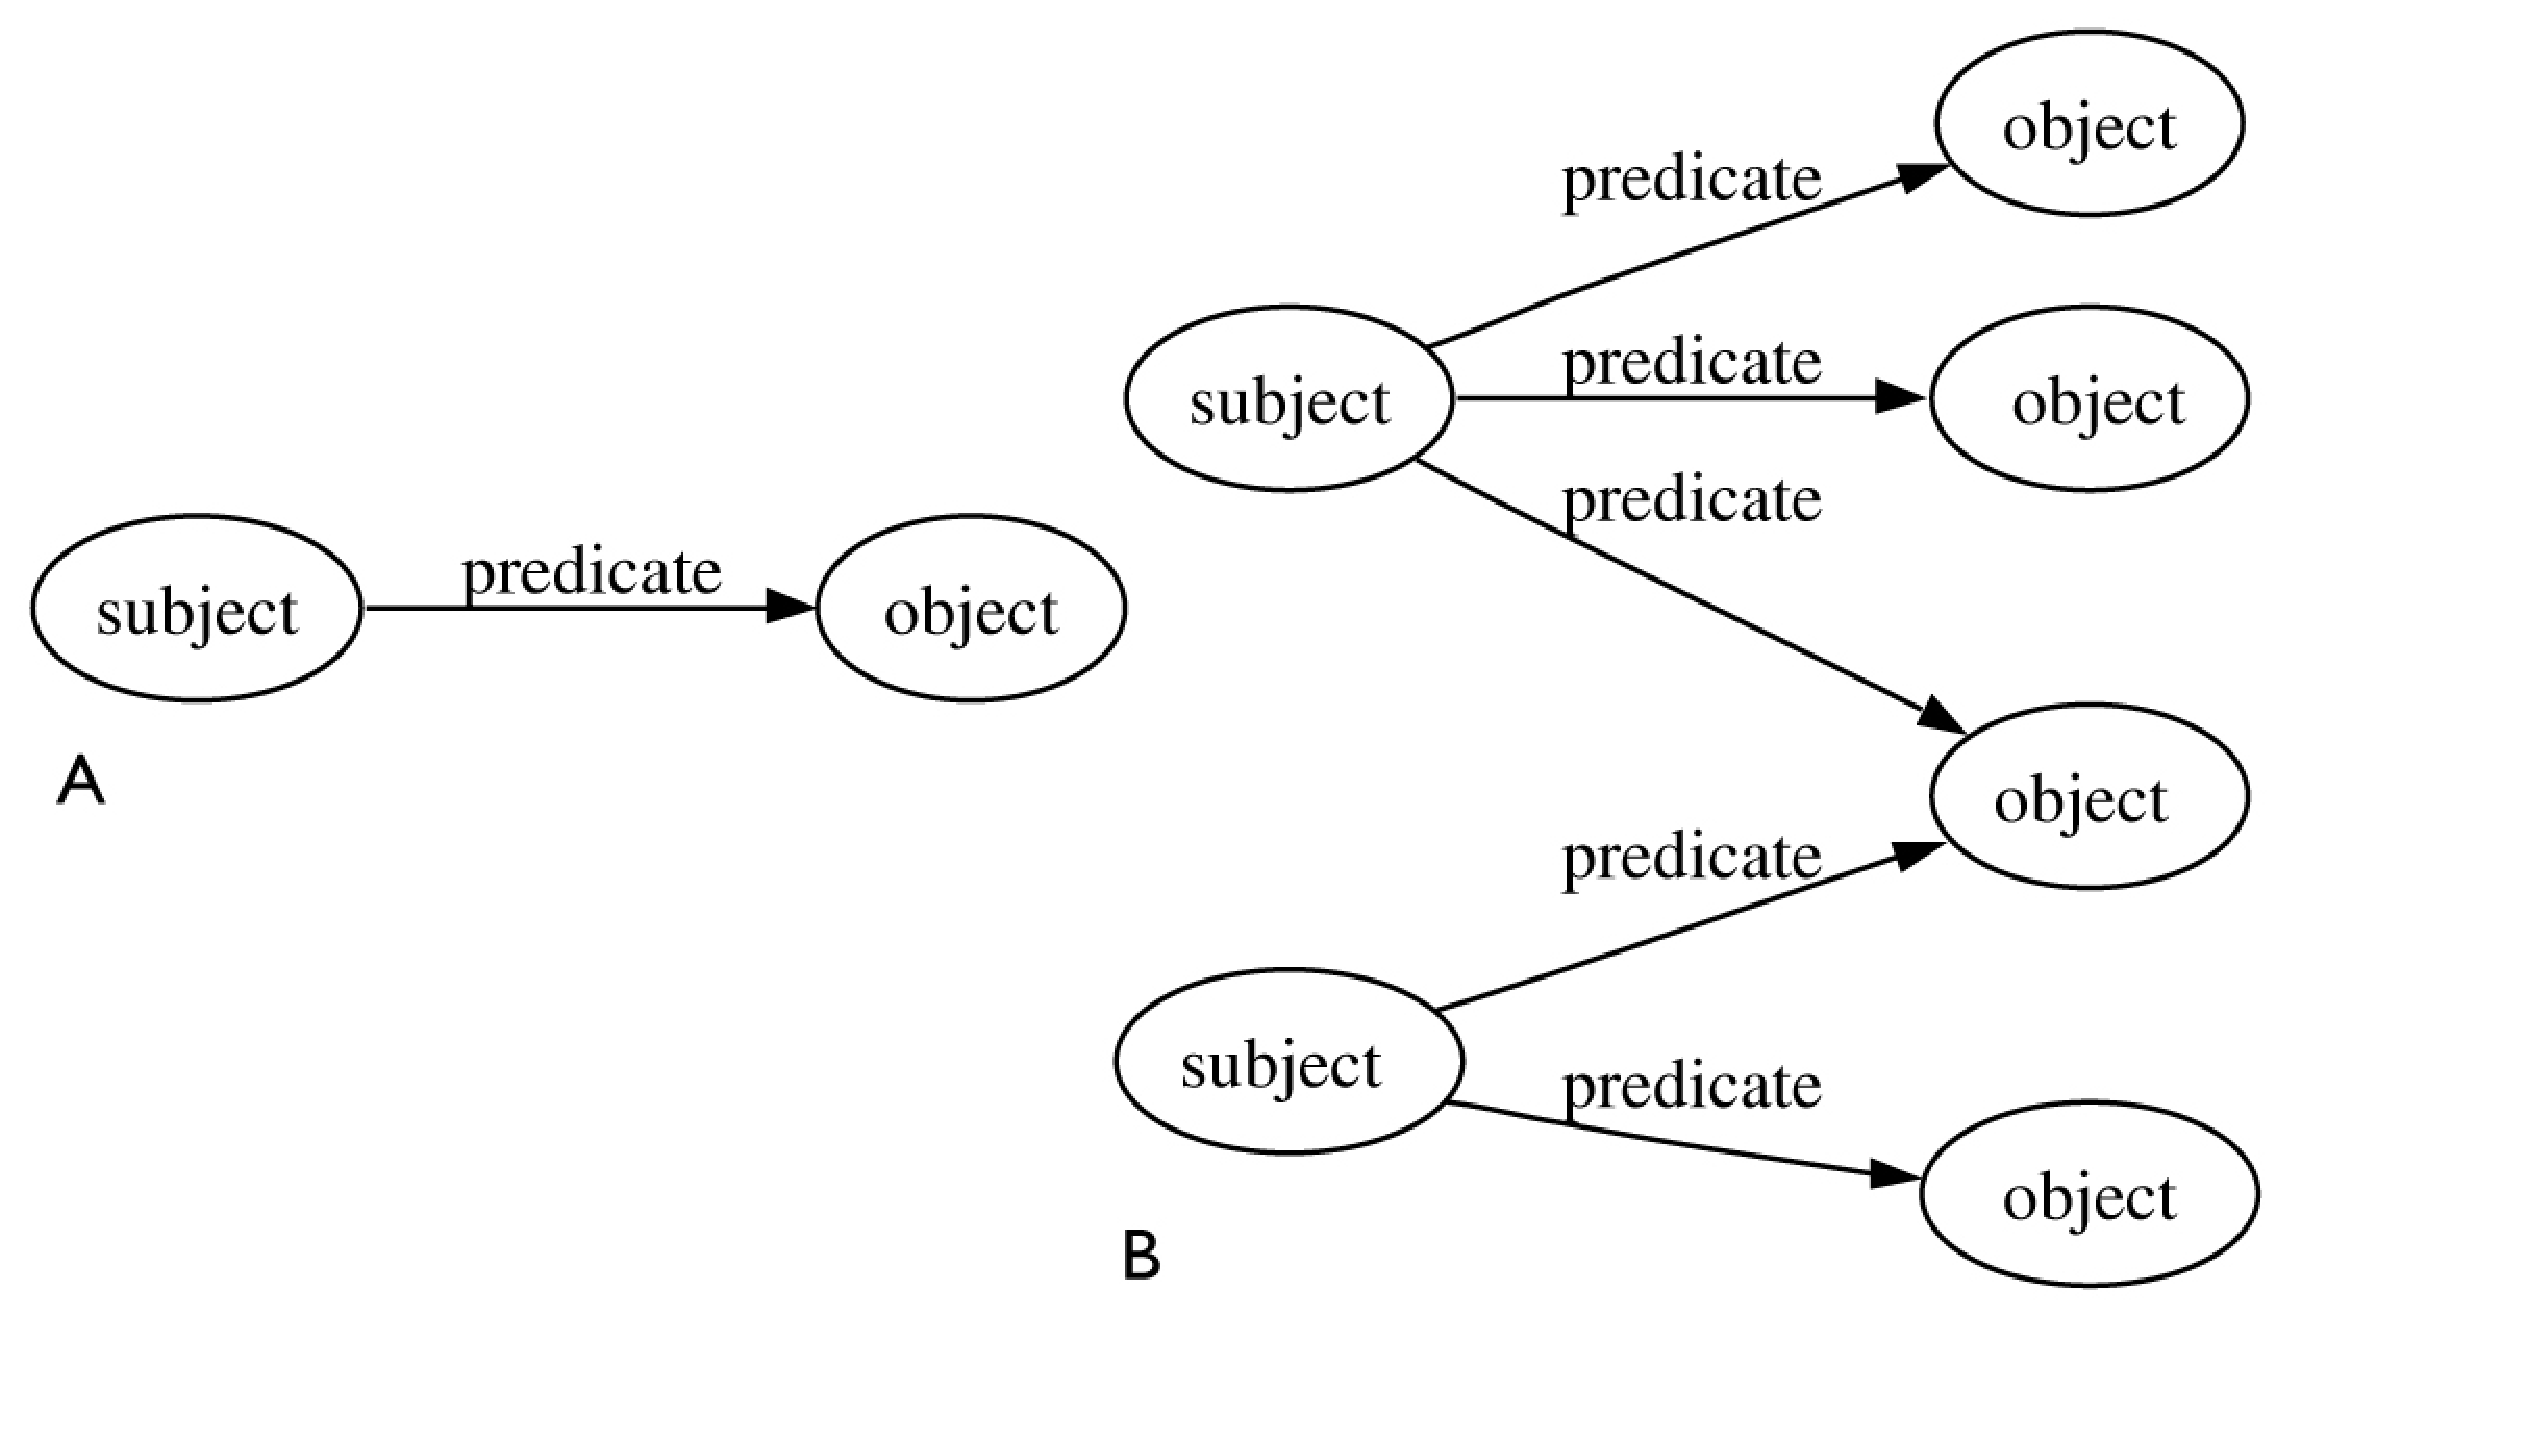
\includegraphics[width=160mm]{./images/rdf_sample.eps}
 		\caption{RDFの例}
 		\label{fig:rdf_triple}
 	\end{center}
\end{figure}

\section{Apache JenaとTDB}

	% 避難場所の使用例
%\chapter{Numerical Examples}
\chapter{数値例と考察}

\section{数値例}

数値例.数値例.数値例.数値例.数値例.数値例.数値例.数値例.
数値例.数値例.数値例.数値例.数値例.数値例.数値例.数値例.
数値例.数値例.数値例.数値例.数値例.数値例.数値例.数値例.
数値例.数値例.数値例.数値例.数値例.数値例.数値例.数値例.


\section{考察}

考察.考察.考察.考察.考察.考察.考察.考察.考察.考察.考察.
考察.考察.考察.考察.考察.考察.考察.考察.考察.考察.考察.
考察.考察.考察.考察.考察.考察.考察.考察.考察.考察.考察.
考察.考察.考察.考察.考察.考察.考察.考察.考察.考察.考察.
	% 関連研究
%\chapter{Main Results}
\chapter{災害発生時に置ける避難場所情報の使用}

\section{避難場所の概要と役割}

避難所は、区市町村があらかじめ指定している避難施設で、災害時等に区市町村長が開設・
管理・運営し、避難者に安全・安心の場として提供することを目的としている.

\section{避難場所情報の検索}

結果-1.結果-1.結果-1.結果-1.結果-1.結果-1.結果-1.結果-1.
結果-1.結果-1.結果-1.結果-1.結果-1.結果-1.結果-1.結果-1.
結果-1.結果-1.結果-1.結果-1.結果-1.結果-1.結果-1.結果-1.
結果-1.結果-1.結果-1.結果-1.結果-1.結果-1.結果-1.結果-1.

\section{数値演算・物の分配}

結果-2.結果-2.結果-2.結果-2.結果-2.結果-2.結果-2.結果-2.
結果-2.結果-2.結果-2.結果-2.結果-2.結果-2.結果-2.結果-2.
結果-2.結果-2.結果-2.結果-2.結果-2.結果-2.結果-2.結果-2.
結果-2.結果-2.結果-2.結果-2.結果-2.結果-2.結果-2.結果-2.

	% 前提知識
%\chapter{Numerical Examples}
\chapter{SIBM - 避難場所情報ベンチマークツール}
\label{sibm_exp}

\section{SIBMの概要・特徴}
\label{sibm:definition}

SIBM(Shelter Information Benchmark)は避難場所情報と避難作業の関係者に関する情報を中心するデータを生成するツールである.

SIBMは以下の2つの目標に基づいて設計されている:

\begin{enumerate}
  \item
  第\ref{info_usage}章に記述した使用シナリオから始め、避難する際、実際に発生する事情を再現できるデータを生成すること。
  \item 拡張性を持つこと:任意の規模を持つデータセットやそのデータの複雑度を選択できることが実験に対する重要な要素であると考えている。
\end{enumerate}

その以外にも、研究分野や使用目的に応じて、様々な場面で活用できることが考えられる。

SIBMでは、避難場所情報を現実に近い情報源を生成する目的を持ち、以下の3つの特徴をもつ:

\begin{itemize}
	\item SIBMでは、指定された避難場所数によるデータを生成することが可能である。
	また、実際の使用例を再現するクエリセットによるベンチマークを行うことで、データベースシステムを評価することができる。
	\item SIBMによる生成した情報の中に、実際の避難場所を使用することや、
	日本人口構成と実際にある人間の関係による関係者情報を生成することで、実際に近い情報源を生成することが可能である。
	\item 避難場所情報・人個人情報・その他の情報(人の就活先・配属情報や外部からのサポートなど)のマッピングによる、実際の情報を再現できる。
\end{itemize}

\section{データ構成の設計}
\label{sibm:data_structure}

SIBMが3つの情報:避難場所情報、関係者の情報とその2つの情報と関係がある他の情報(関係者の所属情報や避難場所の物品情報など)を対象とする。
その3つの要素からなるデータセットが図\ref{fig:sibm_structrure}のように構成される。

避難場所情報が避難場所の詳細情報を表すものである。その構造は以下のようになる(図\ref{fig:sibm_structrure}):

\begin{itemize}
  \item 地上の座標、住所
  \item 収容人数
  \item 災害分類(地震・津波・火山・洪水・その他・未確定)
  \item 施設の種類
\end{itemize}

関係者が3つの種類がある:アシスタント、避難者、ボランチア。関係者全体に対する基本個人情報が生成され、タイプ別に対する情報が追加される。
例えば、ユーザ全体の情報には、ユーザの氏名・年齢・住所・性別などの情報が持つ。
情報共有範囲を管理するために、各タイプそれぞれに対するアクセス可能範囲の情報が追加される。

\begin{figure}[h!]
 	\begin{center}
 		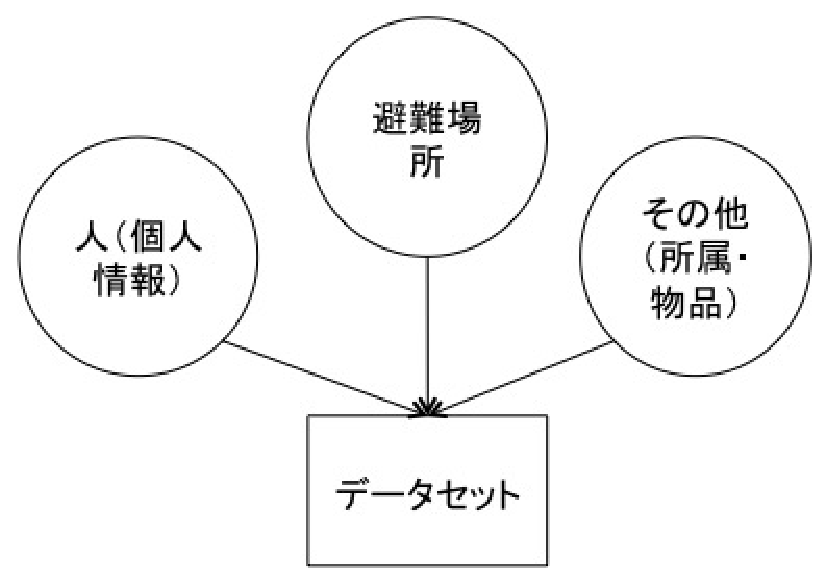
\includegraphics[width=100mm]{./images/sibm_construct.eps}
 		\caption{データセットの構成}
 		\label{fig:sibm_structrure}
 	\end{center}
\end{figure}

関係者の状況・タイプ・年齢などの情報による、所属情報などを生成される。避難場所にたいしては、収容人数情報や面積情報に対する物品情報を追加される。

避難場所情報全体には、避難場所の詳細情報と、その避難場所で避難する・作業する人たちの情報が含まれる。
避難する人や避難場所で作業する人の割合が適切に生成される(図\ref{fig:sibm_shelter})。
また、現実には、災害が発生するとき、一人以上の家族単位で避難することが考えられる。

\begin{figure}[h!]
 	\begin{center}
 		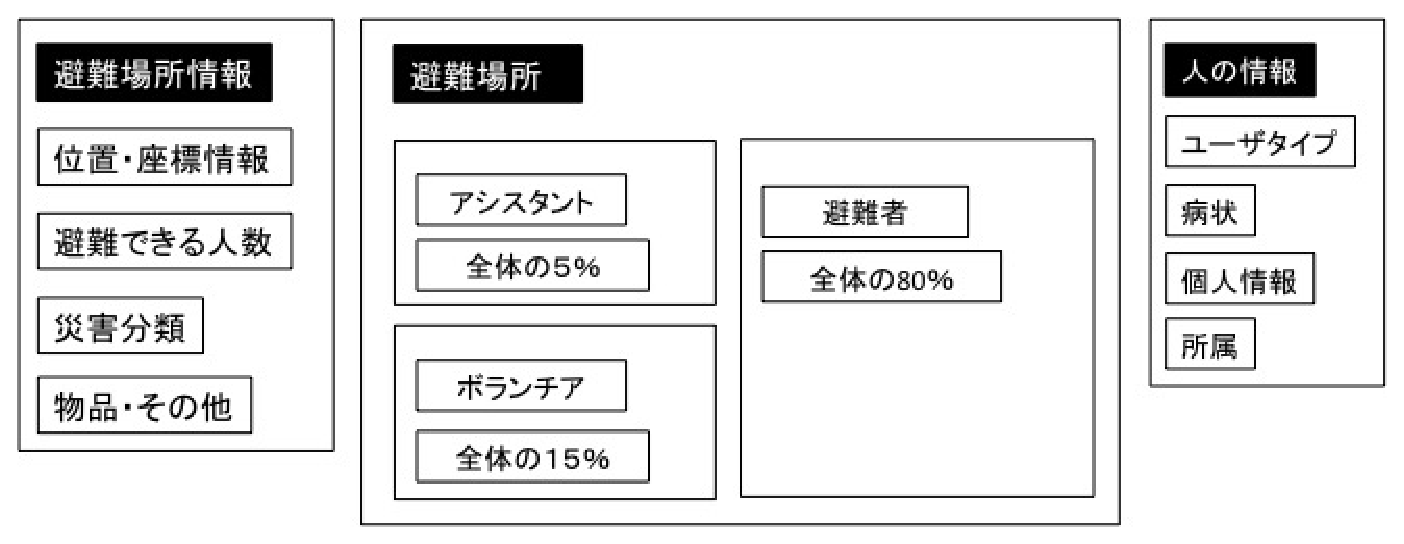
\includegraphics[width=135mm]{./images/sibm_fullimage.eps}
 		\caption{避難場所全体の構成}
 		\label{fig:sibm_shelter}
 	\end{center}
\end{figure}

また、家族全員が違う避難場所で避難することが考えあれ、SIBMでは、そのような関連を追加することが可能である(図\ref{fig:sibm_relationship})。

\begin{figure}[h!]
 	\begin{center}
 		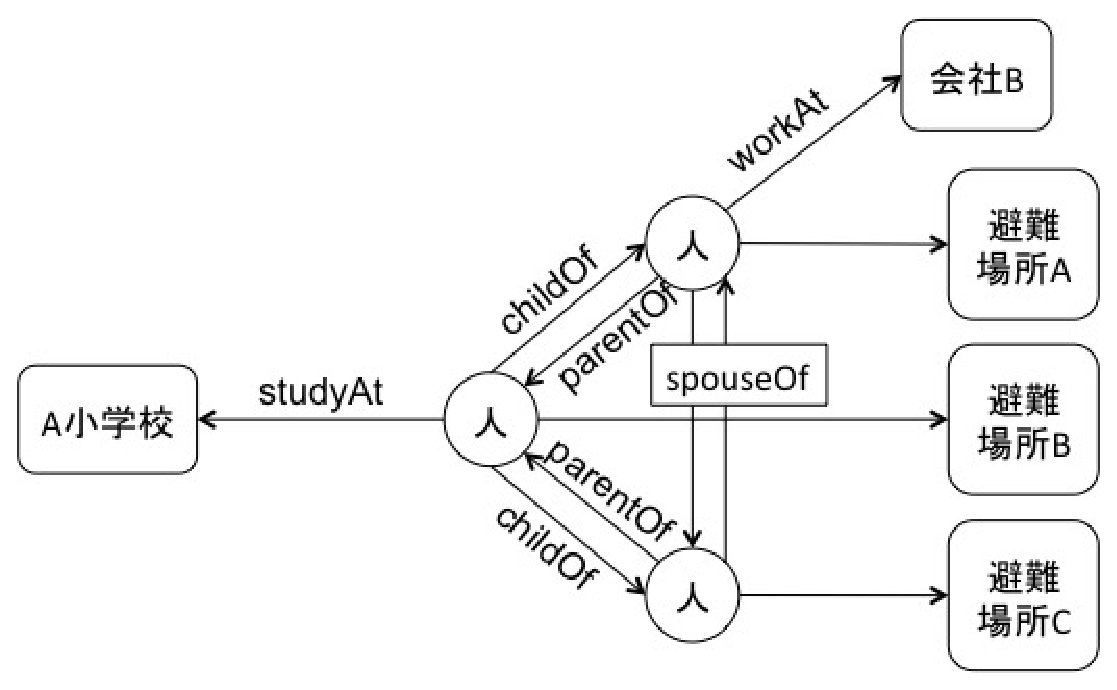
\includegraphics[width=135mm]{./images/sibm_relation.eps}
 		\caption{避難場所に置ける情報構成}
 		\label{fig:sibm_relationship}
 	\end{center}
\end{figure}

最後に、現実のように避難場所が都道府県単位で管理することを表す。
本研究では、平成24年度国土交通省による公開された全国47都道府県の避難場所情報(役12.5万箇所)を使用した。

\begin{figure}[h!]
 	\begin{center}
 		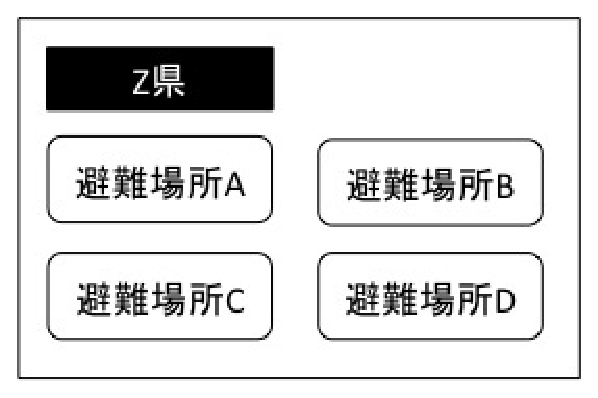
\includegraphics[width=70mm]{./images/sibm_prefecture.eps}
 		\caption{都道府県単位の避難場所構成}
 		\label{fig:sibm_prefecture}
 	\end{center}
\end{figure}

\section{SIBMの実装}
\label{sibm:implements}

\subsection{実装環境}

SIBMがApache Jena(第\ref{knowlegde:top}章)を利用して、Javaプログラミング言語で実装されている。

\subsection{データの生成}

SIBMでは、現実に近い情報を生成する目標を持ち、その目標を実装するために、実際にある情報元を使用することと、実際に近い情報を生成するツールを使用した。
上記の実装を行うための手順や関連するリソースについて以下のように説明する。

\begin{itemize}
	\item
	避難場所情報については、SIBMが\textbf{国土交通省}(MLIT\footnote{Ministry of Land, Infrastructure,
	Transport and Tourism})
	による提供した避難施設情報\footnote{http://nlftp.mlit.go.jp/ksj/index.html}を使用した
	(ただし、最新の情報ではない場合もあることから、災害時に避難施設を利用できることにならない)。
	提供した避難場所情報の詳細が(表\ref{table:data_shelter})になる。
	
	\begin{table}[h]
	\begin{center}
	\begin{tabular}{| l | l | l | p{48mm} |}
		\hline
		\rowstyle{\bfseries}
		データ項目 & フォーマット & 整備年度 & 内容 \\
		\hline
		避難施設 & 点 & 平成24年度 & 位置、行政区域、名称、住所、施設の種類、収容人数、施設規模、災害分類 \\
		\hline
	\end{tabular}
	\caption{避難場所情報の詳細}
	\label{table:data_shelter}
	\end{center}
	\end{table}
	
	また、避難場所の備蓄や、避難場所へのサポート物品・薬品などの情報が避難場所の収容人数や災害発生位置への距離による人口的に生成される。
	最後に、生成された情報をJenaによるRDFデータ形式に出力する。避難場所情報におけるRDFデータの詳細が表\ref{table:data_rdf_predicate}に表示される。
	
	\begin{table}[h]
	\begin{center}
	\begin{tabular}{| l | l | p{48mm} |}
		\hline
		\rowstyle{\bfseries}
		フィルド & RDF述語 & 内容 \\
		\hline
		位置 & geo:geopoint & 避難場所の位置 \\
		\hline
		行政区域 & sibm:administrativeAreaCode &
		都道府県コードと市区町村コードからなる、避難場所の所在する行政区を特定するためのコード \\
		\hline
		名称 & sibm:name & 避難場所の名称 \\
		\hline
		住所 & sibm:address & 避難場所の住所 \\
		\hline
		施設の種類 & sibm:facilityType & 避難場所の分類 \\
		\hline
		収容人数 & sibm:seatingCapacity & 避難施設の形態ごとの収容可能人数 \\
		\hline
		施設規模 & sibm:facilityScale & 避難施設の形態ごとの面積 \\
		\hline
		災害分類 & sibm:hazardClassification & 当該施設が対象とする災害の分類 \\
		\hline
	\end{tabular}
	\caption{避難場所情報のRDF述語の詳細}
	\label{table:data_rdf_predicate}
	\end{center}
	\end{table}

	\item
	人間の情報については、
	SIBMでは、実際の人間の個人情報ではないが、実際に近い情報を生成することができる。
	SIBMが表\ref{table:data_person}のような人間個人情報を生成するツールを構成する。
	構成したツールを使用して人間の個人情報を生成することができ、さらに複雑な情報(家族関係など)を生成することも可能である。
	
	\begin{table}[h]
	\begin{center}
	\begin{tabular}{| l | p{72mm} |}
		\hline
		\rowstyle{\bfseries}
		フィルド & 値 \\
		\hline
		firstName & NLLg \\
		\hline
		surname & Vt \\
		\hline
		gender & Female \\
		\hline
		birthday & 1982-6-5 \\
		\hline
		age & 33 \\
		\hline
		phone & +81xx-xxxx-xxxx \\
		\hline
		email & NLLg\_Vt@Caa.com \\
		\hline
		workAt & 株式会社AAzX \\
		\hline
	\end{tabular}
	\caption{個人情報の例}
	\label{table:data_person}
	\end{center}
	\end{table}
	
	ただし、生成された人中に、男女の割合や年齢の配布が日本人口構造情報による生成される。
	人は家族単位で生成され、家族の「深さ(depth)」パラメーターによる家族の人数が決められる。
	
	例えば、深さ0の家族は一人の場合にあり、3世代の家族まで検討しながら、深さ最大値は2に設定する。
	家族情報を生成する際、最小の子供の年齢から始め、日本人口の「出産平均年齢」の情報
	と「平均子供の数」の情報により、子供の数や親の年齢など家族に関する他の情報を生成する。
	
	最終的に、個人情報の中に、人の年齢、性別、タイプによる所属情報などを生成する。
	
\end{itemize}

生成された避難場所情報は基本的、ある都道府県にある避難場所のリストになり、災害発生位置から離れるような形になる。
実際では、家族の人がなるべく近い避難場所で避難するや作業することが考えられる。そのようなシナリオを実装するために、
生成された家族の人数により、避難場所リストから特定な数だけの避難場所を使用し、家族全員を特定された避難場所に
適切に分配する。

ここまで、避難場所情報・関係者情報及びそれらに関する関連情報を生成することができる。

\subsection{SPARQLクエリセット}

SIBMで生成された情報をクエリすることにより、RDFデータ管理システムを評価することができる。
ここで、第\ref{info_usage}章に説明した避難場所情報の適用シナリオにたいするクエリセットを構成する。

SIBMでは、避難場所情報だけでなく、RDFによる情報を記述したデータも扱う目的を持ち、LUBMを参考したいくつかのRDFデータ構造に対する
クエリを用意する。その一方、第\ref{info_usage}章にある使用シナリオに対するクエリセットも用意する。クエリセットの詳細は付録\ref{appendix1}
に示す。	% SIBM
%\chapter{Numerical Examples}
\chapter{実験・考察}

構成したSIBMを以下の実験環境(表\ref{table:sibm_env})で実装し、データの生成時間やデータベースシステムとのアクセス時間について考察を行う。

\begin{table}[h]
	\begin{center}
	\begin{tabular}{| l  p{45mm} |}
		\hline
		\rowstyle{\bfseries}
		実験環境 & \\
		\hline
		Operation System & Windows 8.1 Pro 64 bits \\
		CPU & Intel core i7 3770, 4 cores 8 thread @ 3.4Ghz (Boostable up to 3.9Ghz)
		\\
		RAM & 16GB \\
		Storage & HDD \\
		Java & 1.7.0\_71 (64 bits) \\
		Apache Jena & 2.12.1 \\
		SIBM & v0.9 build 20150129 \\
		\hline
	\end{tabular}
	\caption{実験環境}
	\label{table:sibm_env}
	\end{center}
\end{table}

SIBMを用いて生成したデータが図\ref{fig:sibm_sample}のような形になる。
	
\begin{figure}[h!]
	\lstinputlisting{./sample/sample.txt}
  	\caption{実装例}
  	\label{fig:sibm_sample}
\end{figure}

大数の避難場所情報を生成する場合、かかった時間やデータ量などの情報が表\ref{table:sibm_time_table}のようになる。

\begin{table}[h!]
	\begin{center}
	\begin{tabular}{| r | r | r | r | r | r |}
		\hline
		\rowstyle{\bfseries}
		避難場所数 & 生成時間(ms) & 関係者数 & トリプル数 & 挿入時間(ms) & サイズ(MB) \\
		\hline
		5 & 3373 & 1455 & 20409 & 3807 & 203.87 \\
		\hline
		10 & 4779 & 3018 & 42304 & 3669 & 205.57 \\
		\hline
		20 & 6783 & 6082 & 85482 & 5588 & 223.91 \\
		\hline
		50 & 7603 & 12645 & 177991 & 8312 & 296.59 \\
		\hline
		100 & 6591 & 24751 & 348443 & 12662 & 379.90 \\
		\hline
		200 & 10363 & 53719 & 755895 & 22522 & 625.34 \\
		\hline
		350 & 24708 & 112888 & 1584015 & 43468 & 1127.90 \\
		\hline
		500 & 30228 & 152903 & 2148284 & 55275 & 1456.53 \\
		\hline
		700 & 42229 & 220201 & 3091954 & 77798 & 2004.87 \\
		\hline
	\end{tabular}
	\caption{避難場所数に対する生成時間}
	\label{table:sibm_time_table}
	\end{center}
\end{table}

図\ref{fig:sibm_data_time}でわかるように、避難場所数が生成時間や人数・トリプル数と比例関係が確認できる。

\begin{figure}[t!]
 	\begin{center}
 		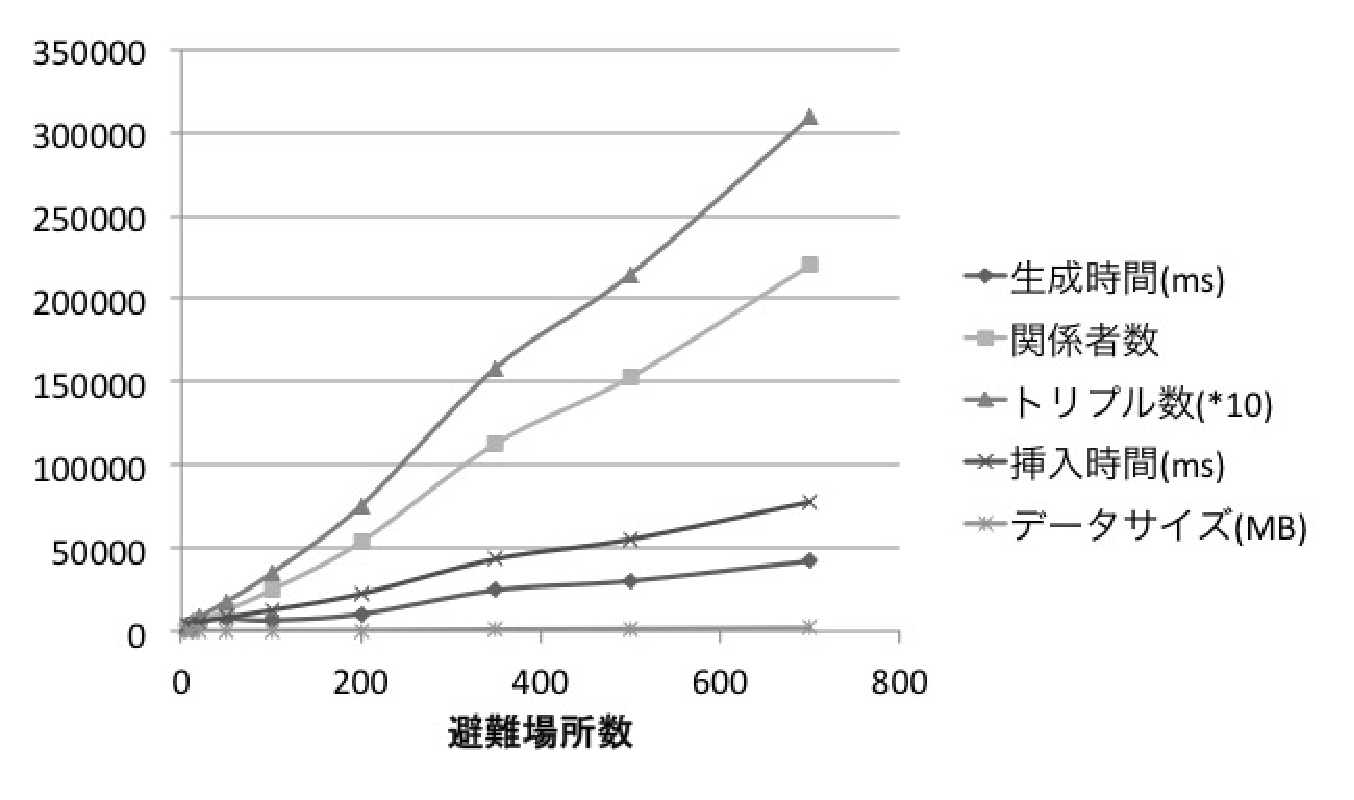
\includegraphics[width=120mm]{./images/test_chart1.eps}
 		\caption{生成・挿入時間とデータサイズ}
 		\label{fig:sibm_data_time}
 	\end{center}
\end{figure}

次に、生成したデータに対するクエリを行い、応答時間につい考察する。
なお、使用したクエリが\ref{appendix1}に説明する。また、Jena/TDBをデータストレージとして使用した。
実行時間をグラフ化した物は以下の図\ref{fig:sibm_query_time}のようになる。

\begin{figure}[t!]
 	\begin{center}
 		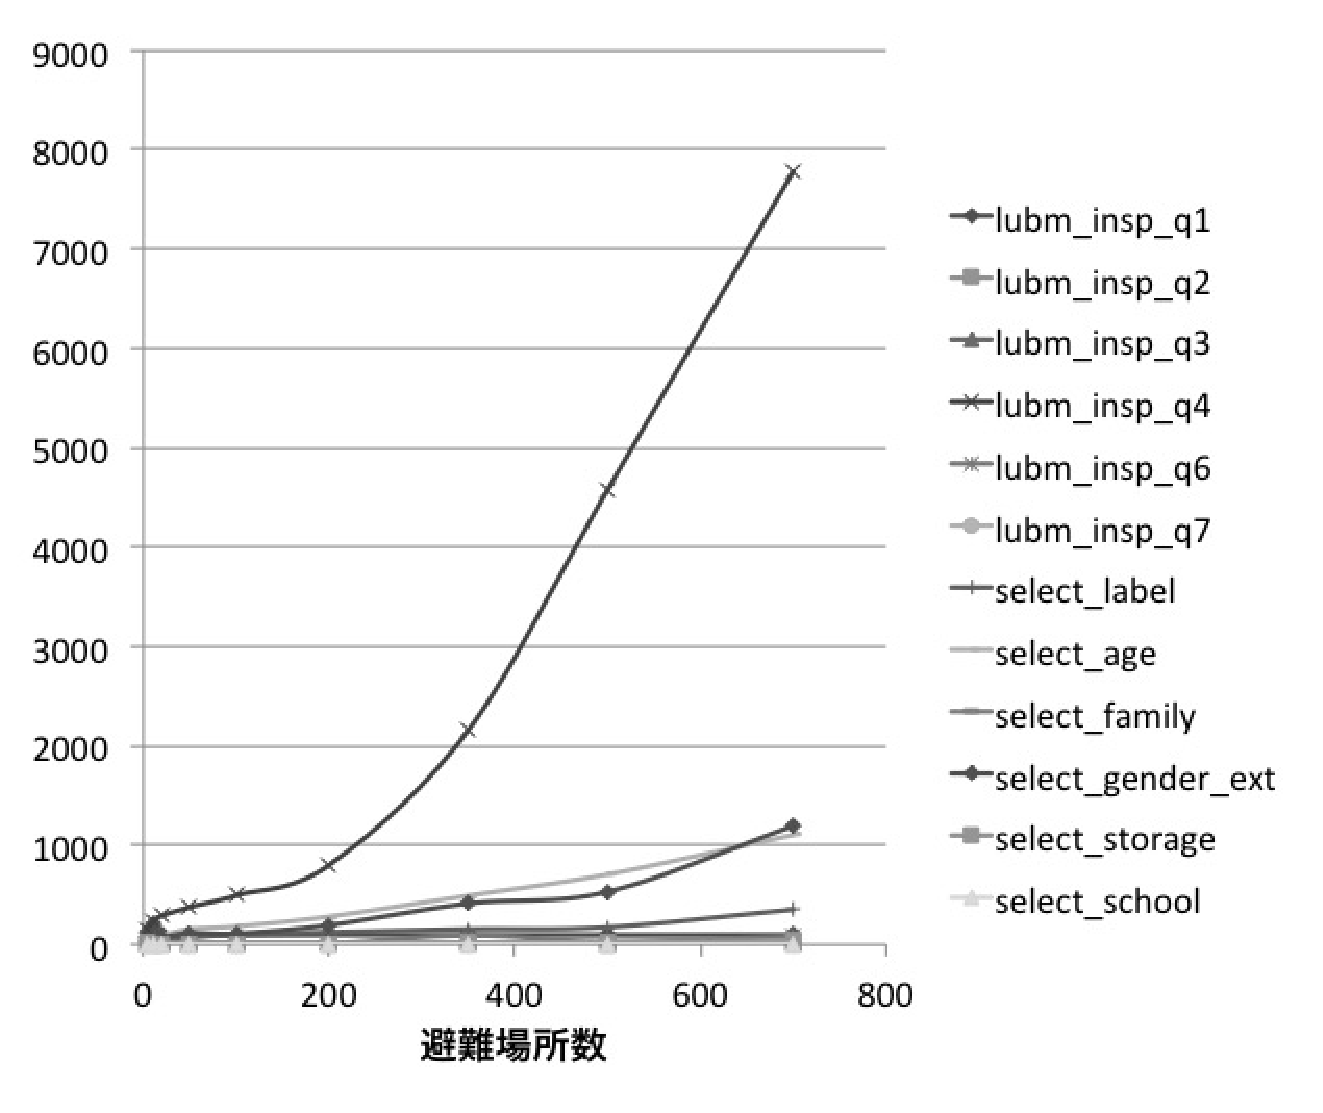
\includegraphics[width=120mm]{./images/test_query1.eps}
 		\caption{クエリ時間}
 		\label{fig:sibm_query_time}
 	\end{center}
\end{figure}

SIBMでは、特定なパラメーターに対する避難場所情報のRDFデータセットを生成することができ、現実に近い情報の元で実験を行うことが可能である。
このセッションでは、SIBMで生成したデータセットとそのもとのパラメーターとの反映性について考察する。また、生成した情報の実用性について考察する。

SIBMバージョン1で対応した入力値は避難場所の数である。SIBMが生成できる最大の数は12.5万となる。
ここでは、生成したデータをJena/TDBデータベースに挿入する時間と挿入後のデータサイズ・トリプル数について考察を行う。
入力した避難場所に対する挿入時間とデータ量が表\ref{table:sibm_time_table}になる。
避難場所の関係者数を避難場所の規模による計算される。その数によって人間情報を生成する。
表\ref{table:sibm_time_table}で示すように、避難場所の数に応じた関係者の数がわかる。

避難場所数とそれに対するデータ生成・挿入時間の関係が図\ref{fig:sibm_data_time}に示す。
生成されたデータ量(関係者数、トリプル数、データサイズ)が避難場所数に対して線形関係があることが考えられる。
だが、トリプル数/避難場所数の関係線が曲線になる。その理由は、特定な避難場所数に対して、生成しようとする関係者の数は定数ではなく、
ある範囲以内でランダムな数値で生成する。関係者情報に対するトリプル数と避難場所情報に対するトリプル数の総数では、ランダム性を持つため、
直線な関係にならないからである。

また、Jena/TDBデータベースでは、挿入するデータに対するメタデータやインデクシングすることによる発生したデータが多い。
そのため、少量データに対してもデータベースサイズが192.0MBになることがわかる\footnote{https://jena.apache.org/documentation/tdb/architecture.html}。

図\ref{fig:sibm_data_time}でわかるように、実際に発生する災害やそれに対する避難情報の増加が問題である。
例えば、北海道には約9000避難場所がある。実際に全てを使用する要求がでると、多量な情報が発生することが考えられる。そして、災害が短時間で発生することが多いため、
その短時間で多量なデータへの対策が事実な問題だとわかる。SIBMで生成するデータを使用し、その問題を解決する候補を実験することができる。
	% 実験・考察
%\chapter{Conclusion}
\chapter{結論・今後の課題}

\section{結論}

世界中に、自然災害による損失や生活への影響を防ぐために、災害対策が重要な問題である。
災害発生時、避難する作業が大切であり、避難する際に関する情報の増加が考えられる。そこで、適切な情報管理システムが求められる。

その一方、近年、災害情報を含め、様々な情報をRDF形式による共有、公開することが多い。そして、RDF形式による、情報の扱いやアクセス制御を
より細かく設計でき、データの管理作業に重要な特徴である。

本研究は、避難場所情報をRDF形式に記述した情報管理システムの評価を位置づけし、災害対策問題に応じる従来の情報管理システムを評価することについて
研究課題とした。そこで、RDF形式で記述した避難場所情報のベンチマークツールを構成することを目的とし、RDFデータ管理システムの評価を始め、
災害対策に応じる実際の避難する作業で発生した使用シナリオをクエリ化することで、現実に近い避難場所情報データセットを生成することを可能にした。

関係者間の関係や避難場所に対する様々な作業を考慮しながら、RDFデータ形式の適用で、従来の求められるシステムへのベンチマークが構成できた。

\section{今後の課題}

構成したベンチマークに対して、いくつかの解決必要な問題が考えられる。

災害発生時、その発生位置から離れる近距離から避難することが考えられる。本研究では、そのようなモデルをもとにして、避難場所を生成することができたが、
避難場所すうの代わりに、災害の強度による避難場所を生成することが現実であろう。そのため、災害強度をパラメーターとして情報を生成することを可能にすることが
今後の課題と設定する。

また、避難場所における事情が時間とともに変動することが事実である。本研究は、そのような変動を再現できず、固定な情報へのアクセスしかできていない。そのため、
情報の歴史や、時間に対する変動な数値に応じる様々な変動に対するベンチマークを構成することを解決すべき課題であると考えている。

最後に、最近よく研究されている多次元情報源やRDFデータにおける各要素の関連(例えば、あるトリプルのSubjectが他のトリプルのObjectとなることなど)がある。
本研究では、そのような関連を人の所属により表現できるが、それに対するクエリなどをつけることはできなかった。従来の管理システムへ向けて、そのような関連を再現できること
が今度の課題とせっていする。
	% 結論・今後の課題
%\chapter*{Acknowledgements}
%\addchapter{Acknowledgements}
\chapter*{謝辞}
\addchapter{謝辞}

皆さんに感謝.皆さんに感謝.皆さんに感謝.皆さんに感謝.
皆さんに感謝.皆さんに感謝.皆さんに感謝.皆さんに感謝.
皆さんに感謝.皆さんに感謝.皆さんに感謝.皆さんに感謝.

%\addchapter{References}
\addchapter{参考文献}
\begin{thebibliography}{9}% 文献数が10未満の時 {9},10~99の時 {99}
\bibitem{cite:opendata}
Jens Ortmann, Minu Limbu, Dong Wang, and Tomi Kauppinen ``Crowdsourcing Linked
Open Data for Disaster Management''

\bibitem{cite:lubm}
Yuanbo Guo, Zhengxiang Pan, and Jeff Heflin ``LUBM: A Benchmark for OWL
Knowledge Base Systems''

\bibitem{cite:kodama}
児玉 快、横田 治夫、``データやユーザの効率的な追加・削除が可能な秘匿情報アクセス手法''

\bibitem{cite:dat}
Vu Tuan Dat、横田 治夫、``MapReduceによる大規模なRDFデータ復号化手法の評価'' 

\bibitem{cite:git_kjs}
M. Fujiwara, ``KSJ - 国土数値情報の変換プログラム'', https://github.com/ma38su/ksj.git

\bibitem{cite:git_data_of_japan}
Data of Japan project, https://github.com/dataofjapan/land.git

\bibitem{cite:jena}
Apache Jena - A Semantic Web Framework for Java, ``https://jena.apache.org''

\end{thebibliography}

\appendix
\chapter{クエリセット}\label{appendix1}

\lstinputlisting[caption=クエリ1,label=q1]{./queries/select_age.rq}

\ref{q1}がお年寄りの問い合わせで検索したクエリである。
% ----------------------------------------------------------------------
\end{document}
